\chapter{Solution}

This chapter describes the complete solution, solving the use cases.
We start with an overview of the solution parts.
Then, we give a detailed description of each part.
\par
The solution consists of four projects, which will form the resulting Blazor website containing PHP scripts.
In Figure \ref{img13:infrastructure}, we can see these projects as green rectangles.
The \textit{Server} project references \textit{Blazor App}, containg a part of the website, and \textit{Peachpie.Blazor}, containing an additional support code.
The server cares about serving the Blazor website and its Static Web Assets.
The next project is our library containing an API for including PHP scripts to the website.
There are \texttt{PhpComponent} and \texttt{PhpScriptProvider}, mentioned earlier, together with additional code support necessary for the correct functionality.
There is the Blazor App project, which becomes the environment for running PHP scripts in a browser.
The project references \textit{PHP scripts} and \textit{Peachpie.Blazor}, which content is used to maintain PHP scripts.
We can see the user's defined scripts as .NET project compiled by Peachpie in \textit{PHP scripts}.
\textit{Blazor App} injects the scripts using the components.
\par
The first section aims at \texttt{PhpComponent}.
It introduces the implementation problems connected to creating render demanding applications and solves them.
The second section talks about \texttt{PhpScriptProvider}.
It suggests a convenient way how to include the scripts into a browser, and it presents the component design.
The last section aims at the server settings.
\par
\begin{figure}[!b]\centering
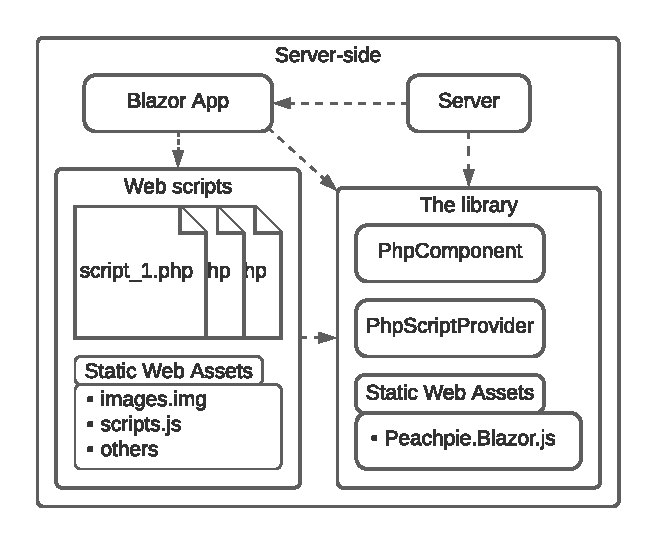
\includegraphics[scale=0.9]{./img/SolutionInfrastructure}
\caption{The solution infrastructure. Green rectangles represent projects. Arrows represent a references.}
\label{img13:infrastructure}
\end{figure} 

\section{PhpComponent}

In the beginning, we introduce problems, which are related to the \textit{PhpComponent} use case.
Then, we suggest a solution and design \texttt{PhpComponent} class.
\par
The first problem causes PHP, which does not know structs and method overloading.
Structs are necessary to work with \texttt{RenderTreeBuilder}, which contains API for adding callbacks handling element events, as we can see in Figure \ref{img14:callback}.
This API uses method overloading in many methods.
\texttt{AddAttribute} is an example where we can write various types of the attribute value.
One of the values can be \texttt{EventCallback} struct representing an event handler.
The struct contains static property \texttt{Factory}, which is a class containing methods for creating callbacks.
\par
\begin{figure}
\begin{lstlisting}
__builder.OpenElement(5, "button");
__builder.AddAttribute(7, "onclick", 
		EventCallback.Factory.Create<MouseEventArgs>((object)this, 
				(Action)IncrementCount));
__builder.AddContent(8, "Click me");
__builder.CloseElement();
\end{lstlisting}
\caption{Fragment of code adding a button element with an event handler.}
\label{img14:callback}
\end{figure}
\par
Peachpie enables using structs in PHP code. 
However, there are limitations at the time of writing, which force us to make workarounds.
We try to rewrite the previous example in PHP code using Peachpie.
We create a component, which inherits {textttComponentBase}. 
Afterward, we override the method for building a render tree and implements the body.
The fragment of the body can be seen in Figure \ref{img15:problems}, where we try using workarounds to make the example functional.
There is the first issue in line 5, where Peachpie does not allow us to access a static property of struct.
It results in a runtime error, which can be solved by \texttt{Helper} written as a C\# class containing a method, which returns the property.
The second issue causes method overloading when Peachpie can not choose the correct version of the \texttt{Create} method in line 8.
Peachpie defines a type of PHP function, \texttt{IPhpCallable}, which can cause the issue
However, if we wrap this function into the correct type by a helper function, the problem remains.
The workaround can be another helper method, which will have a different name for each overload of this method.
However, we come to a compilation error when we want to get an instance of \texttt{EventCallback}.
As we can see in the figure, we tried to use many workarounds, but it is impossible to use some Blazor structures directly in PHP code.
\par
\begin{figure}
\begin{lstlisting}[numbers=left]
use \Microsoft\AspNetCore\Components;
...
$builder->OpenElement(1, "button");
		
//$factory = Components\EventCallback::Factory;
$factory = \ClassLibrary2\Helper::GetFactory();

//$action = function() {\System\Console::WriteLine("Click");}; 
$action = \ClassLibrary2\Helper::GetAction(function() {
	\System\Console::WriteLine("Click");});
		
//$callback = $factory->
//	Create<Components\Web\MouseEventArgs>($this, $action);
$callback = \ClassLibrary2\Helper::
	GetCallback<Components\Web\MouseEventArgs>($factory, 
		$this, $action);

$builder->AddAttribute(2, "onclick", $callback);
$builder->AddContent(3, "Click me");
$builder->CloseElement();
\end{lstlisting}
\caption{Problem of using structs and method overloading. Helper is a class defining workarounds.}
\label{img15:problems}
\end{figure}
\par
To make the example functional, we can hide the struct from PHP code by implementing a C\# helper method using the struct.
The method should have only parameters compatible with PHP types. 
The overloading can be replaced by a different method name for each overload.
Afterward, Peachpie allows us to call the methods from PHP code.
We can use this approach in the \texttt{AddAtribute} method. 
Defining a new method for each overload is a reasonable approach due to a small number of overloads.
Although defining global methods are not the best way, how to do it.
It is a pity that the builder is sealed. 
Although, we can create a wrapper containing the builder and defining method for each overload, which calls the original method in C\# code.
This decision leads us to make a new \texttt{RenderTreeBuilder}  in a different namespace as a wrapper of the original builder.
\par
The next issue relates to rendering time.
\texttt{RenderTreeBuilder} provides a method for adding arbitrary markup text.
The text can contain \texttt{<script>}, but its content is not executed.
At first glance, one can see the method as a convenient way to render the whole content, avoiding using other dedicated methods for building the tree.
These methods accept a sequence number used by the diff algorithm. 
Although using the one method for rendering, the whole component causes slow rendering, which is critical in some applications like games.
The diff algorithm relies on marking the blocks of markup by sequence numbers for optimization in page updates.
When we have only one big block, the diff algorithm can not do anything better than generate an update, which renders the whole page. 
This issue can be seen in the Benchmark section, where we compare the difference between using the one method and utilizing all methods.
Because the builder usage can be complex, we introduce a library for representing tags, helping implement the code using the builder for rendering.
We present library class diagram in Figure \ref{img16:diagram}.
The main idea is to implement the \texttt{iBlazorWritable} interface, which writes the class content into the builder.
An example of a class is \texttt{Tag}, which represents an arbitrary tag.
Because a tag can contain other tags using sequence numbers, we have to keep the currently used sequence number used in the diff algorithm.
For this purpose, the \texttt{writeTreeBuilder} method gets the actual sequence number and returns the last unused number.
This API should hide separated class logics for rendering.
We offer the basic implementation of this method, which renders the content with a dynamic sequence numbering. 
However, a programmer can override the method because sequence numbering is impossible to predefine in advance to make the most effective updates.
Another abstraction is \texttt{AttributeCollerction}, which offers convenient interface for working with attributes by implementing PHP \texttt{ArrayAccess}.
\par
\begin{figure}\centering
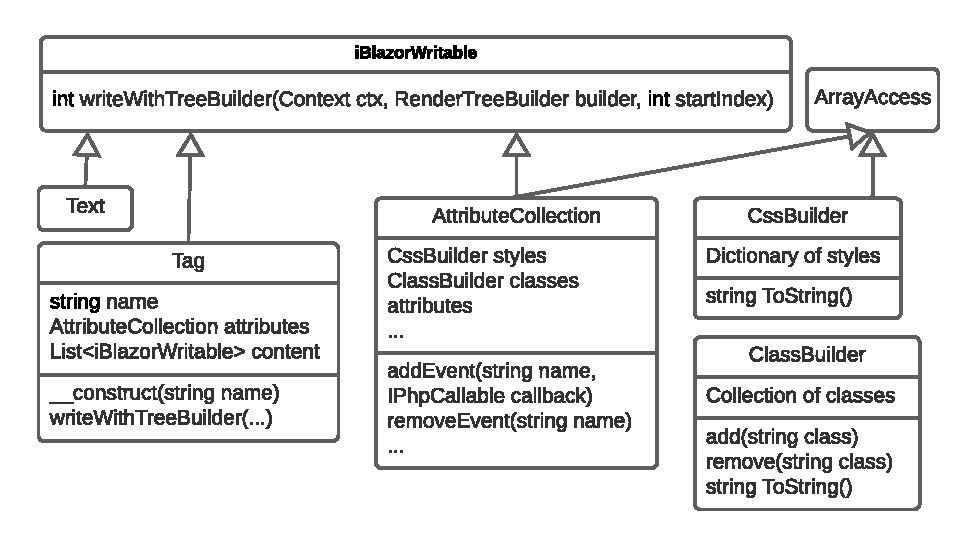
\includegraphics[scale=0.8]{./img/ComponentLibrary}
\caption{Class diagram of supporting library for writting tags.}
\label{img16:diagram}
\end{figure} 
\par
The next barrier is assigning handlers to C\# events in PHP code.
Peachpie does not either support accessing the events.
Thus, we can not directly use a class like \texttt{Timer}, which is useful in \textit{PhpComponent} use case for updating the screen every period.
The issue can be solved by helper methods defined in C\# accepting the object, handler, and event name.
Afterward, we can use reflection for obtaining the desired event by name from the object and then assign the \texttt{IPhpCallable} handler to it.
Because \texttt{Timer} is a common object, we create an additional PHP wrapper class, which uses the timer.
Then a programmer avoids to use the workaround defined above.
\par
\begin{figure}\centering
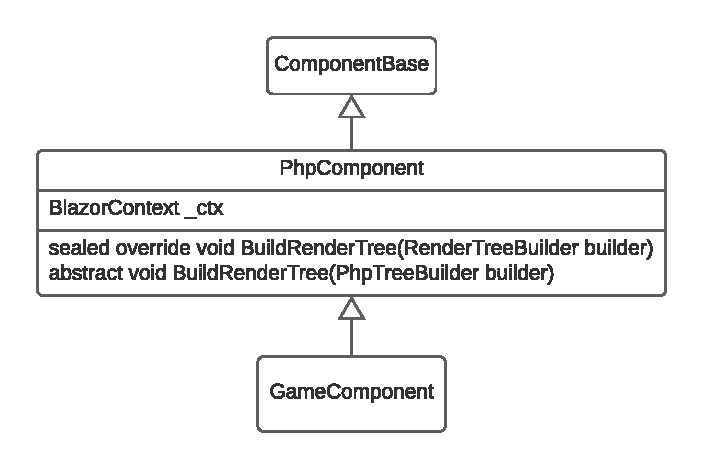
\includegraphics[scale=0.8]{./img/PhpComponentSolution}
\caption{Class diagram of the use case solution.}
\label{img17:solution}
\end{figure}
\par
When we already presented the problems, we can introduce the architecture of \texttt{PhpComponent} and solution of \textit{PhpComponent} use case.
The component hides the original function for rendering and replaces it with our version of the builder, as shown in Figure \ref{img17:solution}.
It results in transparent usage of the builder in the inherited class.
The builder is just a wrapper, so the programmer can use the original builder by accessing its property.
Additional, there is a library for creating tags, which should make the builder usage easier.
For assigning PHP handlers to C\# events, there is a universal helper.
Furthermore, the last feature is a timer wrapper, which uses the C\# timer, offering a convenient API.

\section{PhpScriptProvider}

\change[inline]{Division into functionalities (Router, ScriptProvider, Script)}
\change[inline]{Common things(Script finding,rendering, context, Context save, Using forms, files, parsing url)}
\change[inline]{Router navigating}
\change[inline]{ScriptProvider navigating}
\change[inline]{Script navigating}
\change[inline]{Javascript interop}
\section{Server}
\change[inline]{serving web static assets}